\documentclass[twocolumn, 12pt]{article}
\usepackage[utf8]{inputenc}
\usepackage{amsmath}
\usepackage{marvosym}
\usepackage{textcomp}
\usepackage{geometry}
\usepackage{array}
\usepackage{wrapfig}
\usepackage{multirow}
\usepackage{graphicx}
\usepackage{float}
\usepackage{wrapfig}
\usepackage{caption}
\usepackage{amssymb}
\usepackage{ulem}
\usepackage[table]{xcolor}

\geometry{margin=.5in}

\begin{document}
\small


\section*{Heat Transfer Exam 1}
\begin{equation*}
    q_{cond}'' = -k\frac{dT}{dx}  \hspace{8pt} q_{conv}'' = \overline{h} (T_s-T_{\infty}) \hspace{8pt} q_{rad}'' = \Sigma \sigma (T_s^4 -T_{\infty}^4)
\end{equation*}
\begin{equation*}
    q = q''A    \hspace{15pt}    \sigma \triangleq 5.67 \times 10^-8 \left[\frac{W}{m^2K^4}\right] \hspace{15pt} E = \Sigma \sigma T_s^4
\end{equation*}
\begin{equation*}
     \dot{E}_{in} - \dot{E}_{out} + \dot{E}_g = \dot{E}_{st} \hspace{15pt} \alpha \equiv \text{therm diffusivity} \left[\frac{m^2}{s}\right]
\end{equation*}
\begin{equation*}
    \Sigma q_{in} -\Sigma q_{out} +\dot{q} = \rho Vc_p\frac{\partial T}{\partial t}  \hspace{15pt} \alpha = \frac{k}{\rho c_p}
\end{equation*}
\begin{equation*}
    \frac{\partial}{\partial x}\left( k \frac{\partial T}{\partial x}\right) +\frac{\partial}{\partial y}\left( k \frac{\partial T}{\partial y}\right) +\frac{\partial}{\partial z}\left( k \frac{\partial T}{\partial z}\right) + \dot{q} = \rho c_p \frac{\partial T}{\partial t}
\end{equation*}


\subsection*{Cylindrical}
    \begin{equation*}
        q'' = -k\Vec{\nabla} T = -k\left( \hat{i} \frac{\partial T}{\partial x} + \hat{j} \frac{1}{r}\frac{\partial T}{\partial y} + \hat{k} \frac{\partial T}{\partial z}\right)
    \end{equation*}
    % heat equation
    \begin{center}
    \(
        \rho c_p \frac{\partial T}{\partial t} = 
        \begin{cases}
                    \frac{1}{r} \frac{\partial}{\partial r}\left( kr\frac{\partial T}{\partial r} \right) +\frac{1}{r^2} \frac{\partial }{\partial \phi} \left( k\frac{\partial T}{\partial \phi}\right)\\
                    +\frac{\partial }{\partial z}\left(k\frac{\partial T}{\partial z} \right) +\dot{q}
        \end{cases}
    \)
    \end{center}


\subsection*{Spherical}
    \begin{equation*}
        q'' = -k\Vec{\nabla} T = -k\left( \hat{i} \frac{\partial T}{\partial r} + \hat{j} \frac{1}{r}\frac{\partial T}{\partial \theta} + \hat{k} \frac{1}{rsin(\theta)} \frac{\partial T}{\partial \phi}\right)
    \end{equation*}
    % Heat equation
    \begin{center}
    \(
        \rho c_p \frac{\partial T}{\partial t} = 
        \begin{cases}
                        \frac{1}{r^2} \frac{ \partial }{\partial r}\left( kr^2 \frac{\partial T}{\partial r} \right) + \frac{1}{r^2sin^2(\theta)} \frac{\partial }{\partial \phi }\left(k\frac{\partial T}{\partial \phi} \right) \\
                        + \frac{1}{r^2 sin(\theta)} \frac{\partial }{\partial \theta}\left(ksin(\theta)\frac{\partial T}{\partial \theta} \right) + \dot{q}
        \end{cases}
    \)
    \end{center}

    

\subsection*{Thermal Resistance \(\dot{q}=0\)}
{\renewcommand{\arraystretch}{2}
\begin{tabular}{l|c|c|c}
                & Conduction & Convection & Radiation \\
     \hline
     Plane Wall & \(R_t = \frac{L}{kA}\) & \(R_t=\frac{1}{hA}\) & \(R_t =\frac{1}{h_RA}^*\)\\
     \hline
     Cylindrical & \(ln\left(\frac{r_2/r_1}{2\pi Lk}\right)\) & &\\
     \hline
     Spherical &  \(\frac{\left(\frac{1}{r_1}-\frac{1}{r_2} \right)}{4\pi k}\) & &
\end{tabular} \quad}
\begin{center}
    * \(h_R = \varepsilon \sigma (T_s+T_{sur})(T_s^2+T_{sur}^2)\)
\end{center}
\begin{equation*}
    R_{t,contact} = \frac{T_A-T_B}{q_x} \hspace{20pt} R_{t,contact}'' = \frac{T_A-T_B}{q_x''}
\end{equation*}
\begin{equation*}
    R_{tot} = \Sigma R_t \hspace{15pt} q_x = \frac{T_{bigger}-T_{smaller}}{R_{tot,between}}
\end{equation*}



\subsection*{Alternate Conduction \(\dot{q} =0\)}
    \begin{itemize}
        \item Plane Wall
                \begin{equation*}
                    q_x = \int^{x_f}_{x_0} \frac{dx}{A(x)} = - \int^{T_f}_{T_0}k(T)dT
                \end{equation*}
                \begin{center}
                    Heat rate and heat flux are constant.
                \end{center}
        \item Cylindrical 
                \begin{equation*}
                    q_r = -k(2\pi rL) \frac{dT}{dr} = \frac{T_{s1}-T_{s2}}{\frac{ln(r2/r1)}{2\pi Lk}}
                \end{equation*}
                \begin{center}
                    Heat rate is constant. Heat flux is \textbf{NOT}
                \end{center}
                \begin{equation*}
                    T(r)=\frac{T_{s1}-T_{s2}}{ln(r2/r1)} \hspace{5pt} ln\left(\frac{r}{r_2}\right) + T_{s2}
                \end{equation*}
                
        \item Spherical
                \begin{equation*}
                    q_r = \frac{T_{s1}-T_{s2}}{\left(\frac{1}{r_1}-\frac{1}{r_2}\right)/4\pi k} = -4 k\pi r^2 \frac{dT}{dr}
                \end{equation*}
                \begin{center}
                    Heat rate is constant. Heat flux is \textbf{NOT}
                \end{center}
    \end{itemize}

    
    


\subsection*{Fins}
    \begin{center}
        1D, steady-state, \(\dot{q}=0\), constant properties
    \end{center}
    \begin{equation*}
        \frac{d^2T}{dx^2} + \left(\frac{1}{A_c}\frac{dA_c}{dx} \right)\frac{dT}{dx} -\left( \frac{1}{A_c} \frac{h}{k} \frac{dA_s}{dx} \right)(T-T_\infty) = 0
    \end{equation*}
    \begin{equation*}
        \text{if const. } A_c \hspace{5pt} \bigwedge \hspace{5pt}\theta(x) \triangleq T(x)- T_\infty \text{  then:}
    \end{equation*}
    \begin{equation*}
        \frac{d^2\theta}{dx^2} - m^2\theta(x) =0 \hspace{20pt} m = \sqrt{\frac{hP}{kA_c}}
    \end{equation*}
    \begin{equation*}
        \varepsilon_f = \frac{q_f}{hA_{c,b}\theta_b} = \frac{\text{fin heat rate}}{\text{heat rate w/o fin}} = \sqrt{\frac{kP}{hA_c}}
    \end{equation*}
    \begin{equation*}
        \varepsilon_f = \frac{R_{t,b}}{R_{t,f}} = \frac{\text{resist. @ base w/o fin} \because \text{conv.}}{\text{max heat rate if all rod @ }T_b}
    \end{equation*}
    \begin{equation*}
        \eta_f = \frac{q_f}{q_{max}} = \frac{q_f}{hA_f,\theta_b}=\frac{\text{fin heat rate}}{\text{max rate if all rod @ } T_b}
    \end{equation*}
    \begin{equation*}
        \eta_f = \frac{tanh(L_c)}{mL_c} \hspace{8pt} \square \rightarrow L_c = L +t/2 \hspace{8pt} \bigcirc \rightarrow L_c = L+D/4 
    \end{equation*}
\subsection*{Finite Difference Equations}
\begin{enumerate}
    \item Pick the node you care about, it is node (m,n)
    
    \item Determine \(q\) from surrounding nodes (pointed towards node m,n)
    
    \item Do an energy balance, solve for \(T_{(m,n)}\)
\end{enumerate}



\subsection*{Lumped Capacitance Method}
    Check Biot number first, \textbf{if} \(Bi<0.1\), L.C.M. is valid. 
    \begin{equation*}
        Bi \triangleq \frac{hL_c}{k} \hspace{12pt} L_{c,plane} = L \hspace{12pt} L_{c,cyl} = \frac{r_o}{2}  \hspace{12pt} L_{c,sph} = \frac{r_o}{3} 
    \end{equation*}
    \begin{equation*}
        t = -\frac{\rho V c}{hA_s} ln\left(\frac{\theta}{\theta_i}\right) \hspace{10pt} \tau_t = \rho V c \frac{1}{hA_s} = C_t R_t \hspace{10pt} L_c = \frac{V}{A_s}
    \end{equation*}
    \begin{equation*}
        \frac{\theta}{\theta_i} = \frac{T-T_\infty}{T_i-T_\infty} = exp\left(-\frac{hA_s}{\rho V c} t \right) = exp(-Bi\cdot Fo)
    \end{equation*}
    \begin{equation*}
        Fo = \frac{\alpha t}{L_c^2}= \frac{k t}{\rho c_p L_c^2} \hspace{15pt} Q = \rho Vc (T_i-T_\infty)(1-e^{-t/\tau}) \hspace{3pt} [J]
    \end{equation*}
    

\subsection*{Spatial Effects}
\begin{itemize}
    \item If \(Bi \nless 0.1\), take into account spatial effects (Use the \(Bi\) formula listed at the bottom of the table). 
    \item Assume \(Fo > 0.2\), to use the single term approximation. If \(Fo \ngtr 0.2\), the infinite series must be dealt with. \textbf{Good luck.}
\end{itemize}
    \begin{equation*}
        \theta^* \triangleq \frac{\theta}{\theta_i} = \frac{T-T_\infty}{T_i-T_\infty} \hspace{20pt} 0\leq \theta^* \leq 1 \hspace{20pt} \frac{\partial^2 \theta^*}{\partial x^{*2}} = \frac{\partial \theta^*}{\partial Fo}
    \end{equation*}
    \begin{equation*}
        x^*\triangleq \frac{x}{L} \hspace{20pt} 0\leq x^* \leq 1 \hspace{20pt} t^* = Fo =\frac{\alpha t}{L_c^2}
    \end{equation*}
    \begin{equation*}
        \theta^* = \sum_{n=1}^\infty C_n exp(-\zeta_n^2 Fo)cos(\zeta_n x^*) \hspace{10pt} C_n = \frac{4sin(\zeta_n)}{2\zeta_n + sin(2\zeta_n)}
    \end{equation*}
    \begin{center}
        Approximate solution (1-term) is only valid for symmetric, or adiabatic on one side
    \end{center}
    \begin{equation*}
        \theta_0^* = C_1 exp (-\zeta^2_1 Fo) = \frac{T-T_\infty}{T_i-T_\infty} \hspace{8pt} (\theta_0^* \text{  is midplane of }\theta^*)
    \end{equation*}
    \begin{equation*}
        \theta^* = \theta_0^* cos(\zeta_1 x^*)
    \end{equation*}
    
    
    \subsection*{Locations of Appendices and Tables}
    \begin{tabular}{|l|l|l|}
        \hline
        \rowcolor{lightgray}
        Fin temp table & Table 3.4 & pg 161 \\
        \hline
        Finite Diff. Equations & Table 4.2 & pg 246\\
        \hline
        \rowcolor{lightgray}
        Spatial effects coeff. & Table 5.1 & pg 301 \\
        \hline
        Thermophysical props. & Appendix A & pg 981\\
        \hline
        \rowcolor{lightgray}
        Zeta values for \(\zeta_1 - \zeta_4\) & Appendix B.3 & pg 1016\\
        \hline 
        Bessel Functions  & Appendix B.4 & pg 1017\\
        \hline 
        \rowcolor{lightgray}
        Heat generation eq's & Appendix C & pg 1019\\
        \hline
    \end{tabular}
    
    
    \begin{figure}[h!]
        \centering
        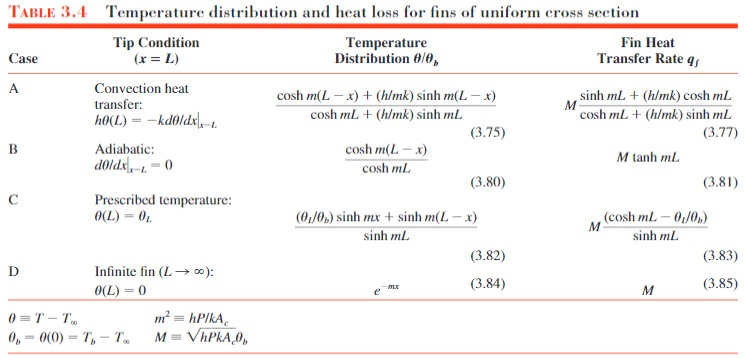
\includegraphics[scale = 0.58]{Table3_4.jpg}
    \end{figure}
    \begin{figure}[h!]
        \centering
        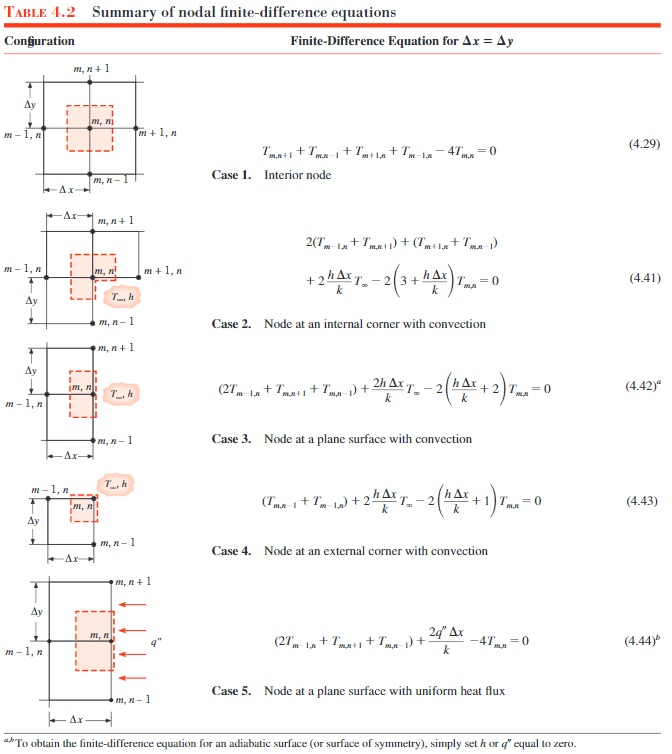
\includegraphics[scale=0.6, angle=90]{Table4_2.jpg}
    \end{figure}
    \begin{figure}[h!]
        \centering
        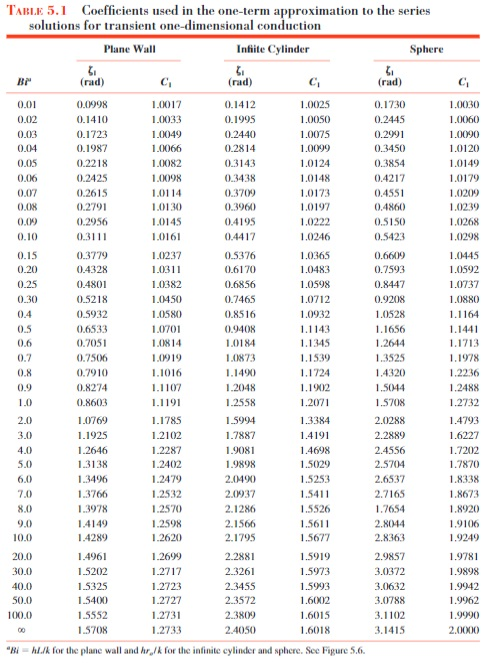
\includegraphics[scale = 0.8]{Table5_1.jpg}
    \end{figure}
    %\begin{figure}[h!]
     %   \centering
     %   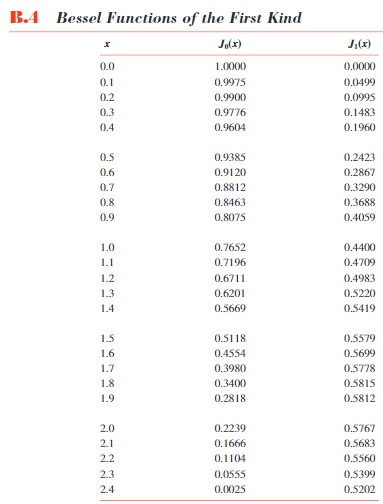
\includegraphics[angle=90, scale=0.7]{AppendixB_4.jpg}
    %\end{figure}


\end{document}